\chapter{SYSTEM ANALYSIS AND DESIGN}
\section{System Analysis}
The project is following a structured approach that utilizes the Rapid Application Development (RAD) methodology. This approach segments the project into smaller, manageable components, allowing for incremental progress through iterative development. Individual modules are developed and integrated progressively, focusing on delivering and refining smaller segments. This method ensures continuous improvement and alignment with the overall goals while effectively managing the project through ongoing feedback and adjustments.
\subsection{Requirement Analysis}
Requirement analysis is a critical phase in the software development lifecycle that focuses on understanding and documenting the needs and expectations of stakeholders. This process involves gathering detailed information about what users require from a system, which includes identifying functional requirements (what the system should do), non-functional requirements (how the system should perform), and constraints (limitations or restrictions). The goal is to create a comprehensive and clear specification that guides the development team in designing and implementing the system. Effective requirement analysis ensures that the final product aligns with user needs and business objectives, reduces the risk of project failure, and facilitates efficient communication among stakeholders. By thoroughly analyzing requirements, teams can address potential issues early, prioritize features, and ensure a smoother development process.
\subsubsection{Functional Requirements}The functional requirements of LabXplorerX are mentioned below:
\begin{itemize}
    \item \textbf{User Profiles:}  
    LabXplorerX allows children and teachers to create personalized profiles for managing their activity within the platform. Users can log in with unique credentials. The profile section displays only the user's own comments and interactions within the platform, along with a list of their favorited capsules. This streamlined approach helps users easily track their contributions and revisit their most valued content.

    \item \textbf{Interactive Virtual Simulations:} LabXplorerX offers a range of interactive virtual simulations, including Basic Electronics, Basic Chemistry, Basic Astronomy, and an Online Coding Environment. These simulations provide immersive experiences where users can engage in hands-on activities, such as manipulating virtual equipment and conducting experiments. By integrating interactive animations and real-world scenarios, LabXplorerX facilitates experiential learning, allowing users to explore scientific principles and phenomena in a dynamic digital environment.

    \item \textbf{Capsule Tools:}  
    In LabXplorerX, only administrators have the ability to create educational capsules, quizzes, and simulation links. They can design capsules with interactive quizzes, organize educational content. However, the creation and development of new simulations are restricted to developers, ensuring that complex interactive simulations are handled by technical experts while allowing administrators to manage and assign tasks within the platform.
    

    \item \textbf{Comments and Favourites for Learning Capsules:}  
    LabXplorerX provides a comments section for each learning capsule, allowing students and teachers to leave feedback, ask questions, or share insights directly related to the content. Users can engage with one another by commenting on specific capsules. Additionally, the platform supports a "favourites" feature, enabling users to bookmark and easily revisit their preferred capsules, enhancing their personalized learning experience.


    \item \textbf{Quizzes and Learning Capsules:} LabXplorerX integrates quizzes and learning capsules to reinforce knowledge and assess comprehension. Quizzes are designed to evaluate understanding of concepts covered in simulations, while learning capsules provide bite-sized, focused content on specific topics. These features help consolidate learning and provide instant feedback.

    \item \textbf{Admin Dashboard:}  
    The admin dashboard in LabXplorerX provides a centralized interface for managing user accounts, monitoring platform usage, and overseeing system performance. Administrators have the ability to perform full CRUD (Create, Read, Update, Delete) operations on quizzes and capsules, ensuring content is up-to-date and relevant. They can also add simulation links to capsules, making it easier to integrate simulations into the learning experience, while maintaining control over the platform's content and functionality.

\end{itemize}

\begin{figure}[H]
    \centering
     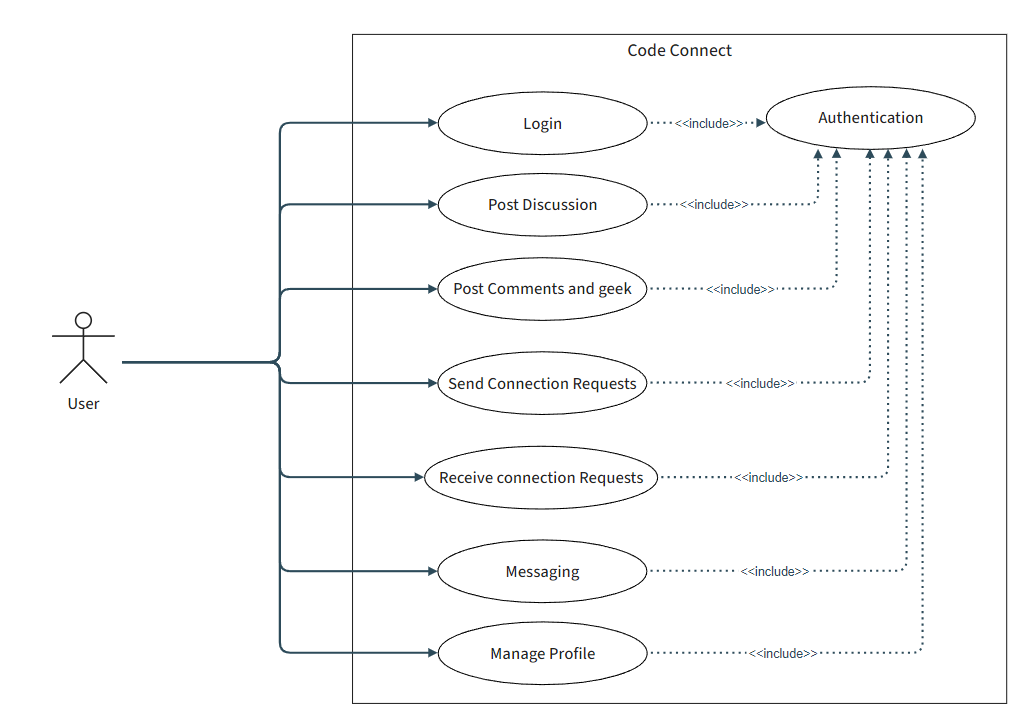
\includegraphics[height = 12cm]{Diagrams/use_case.png}
     \caption{Use Case Diagram}
 \end{figure}

\subsubsection{Nonfunctional Requirements}
The nonfunctional requirements of LabXplorerX are mentioned below:
\begin{itemize}
    \item \textbf{Performance Enhancement:} The focus on performance involves optimizing the platform to handle high user loads and complex simulations efficiently. This includes minimizing reliance on external frameworks and ensuring smooth and responsive interactions.
    \item \textbf{Authentication Security:} Security is a paramount concern. To enhance the platform’s security, advanced authentication algorithms, particularly focusing on hashing techniques within the backend environment, have been implemented. This ensures that user authentication data is stored and managed in a highly secure manner.
    \item \textbf{Better UX Design:} User experience is central to the project’s success. The emphasis on better UX design means that every aspect of the platform’s interface, from navigation to interaction, will be meticulously crafted to ensure a seamless and intuitive experience. This design approach caters not only to experienced users but also to newcomers, ensuring that all users can effortlessly navigate and engage with the platform.
    \item \textbf{Responsive Design:}  
    Recognizing the diverse range of devices and browsers used by users, the platform features a responsive design that ensures optimal adaptation across different screen sizes for most interface elements. This means that users can effectively access and interact with the platform whether they are using a desktop computer, tablet, or smartphone. However, it's important to note that the simulations are not responsive and are limited to desktop use. This approach guarantees a consistent and satisfying experience on various devices for general content, while simulations remain optimized for desktop environments.

\end{itemize}
\section{Feasibility Analysis}
A feasibility study is a systematic and structured analysis conducted to determine the viability and practicality of a proposed project plan. It serves as an evaluation tool to assess whether the project can be successfully implemented and if it aligns with the organization's goals and objectives. It involves gathering and analyzing relevant information to determine if the project is technically feasible, operationally feasible, economically feasible, and scheduling feasible.
\subsection{Economical Feasibility}
The development of the web application will utilize a range of free and open-source software development tools. For the frontend, React, a popular JavaScript library for building dynamic and interactive user interfaces, will be used. On the backend, Express, a minimal and flexible Node.js web application framework, will handle server-side logic and HTTP requests. PostgreSQL, an open-source relational database management system known for its reliability and performance, will be employed for database management. Interactive simulations will be created using Phaser, a robust HTML5 game framework, while Unity, a powerful cross-platform game engine, will be used for more complex simulations and 3D elements. Additionally, funds will be allocated for economical server hosting to ensure the application remains accessible to users while managing costs effectively.
\subsection{Operational Feasibility}
LabXplorerX prioritizes operational feasibility through a user-centric design approach, emphasizing simplicity and ease of use. The system is highly interactive, enabling both students and educators to navigate effortlessly without requiring extensive technical knowledge. The user interface (UI) features a clean layout and intuitive controls, ensuring a seamless experience when accessing virtual environments and educational resources. By minimizing the need for extensive training and reducing potential barriers to adoption, LabXplorerX enhances user acceptance and engagement. The straightforward design promotes effective use of the app's features, supports educational activities, and fosters a positive user experience.
\subsection{Technical Feasibility}
Combining Express.js with React and PostgreSQL offers a robust and scalable solution for developing modern applications. Express.js, built on Node.js, provides an efficient backend framework for creating RESTful APIs and managing server-side logic. PostgreSQL, known for its reliability and advanced data management features, serves as a solid foundation for secure and efficient data storage and querying. On the frontend, React facilitates the creation of responsive and visually appealing applications across multiple platforms using a single codebase. This stack leverages the strengths of each technology: Express.js for backend scalability and API development, PostgreSQL for comprehensive data handling, and React for seamless and dynamic UI development. Supported by active communities and extensive documentation, this combination ensures ample technical support, resources, and flexibility for both deployment and maintenance, making it an ideal choice for delivering modern, interactive applications.
\section{Structured System Modelling }
Structured system modeling is a methodical approach used to design complex systems by decomposing them into manageable components and utilizing formal diagrams and tools. This approach aids in clearly defining system requirements, workflows, and interactions. By breaking down a system into its constituent parts, structured system modeling facilitates a thorough understanding of its structure and behavior. The use of formal diagrams and tools ensures that all aspects of the system are documented and analyzed systematically, which enhances clarity, communication, and accuracy throughout the design process. This methodical approach supports the creation of well-organized and efficient systems, improving overall design quality and project outcomes.
\newpage
\subsection{Process Modeling : DFD}
Processing Modeling visually represent the flow of processes within a system, showing how data are flowed from external entites to processes. This mainly deals with what is the system rather than how. These can be done through Data Flow Diagrams. These DFD are not the technical side rather an Representation of what the system does.\\
\textbf{Context Level DFD}\\
This is also known as Level 0 DFD which shows overall flow of data into system as a whole.
\begin{figure}[H]
    \centering
        
\includegraphics[height = 4cm]{Diagrams/ProcessModelling.png}
    \caption{Process Model: DFD (Context Level)}
\end{figure}
\vspace{-1em}
\textbf{Level 1 DFD}\\
This is also known as Level 1 DFD which shows flow of data into system and its Major Processes.Here it has diffrent Process like Simulation System,User Management etc with their respective numbers 1.0, 2.0 etc.
\begin{figure}[H]
    \centering
        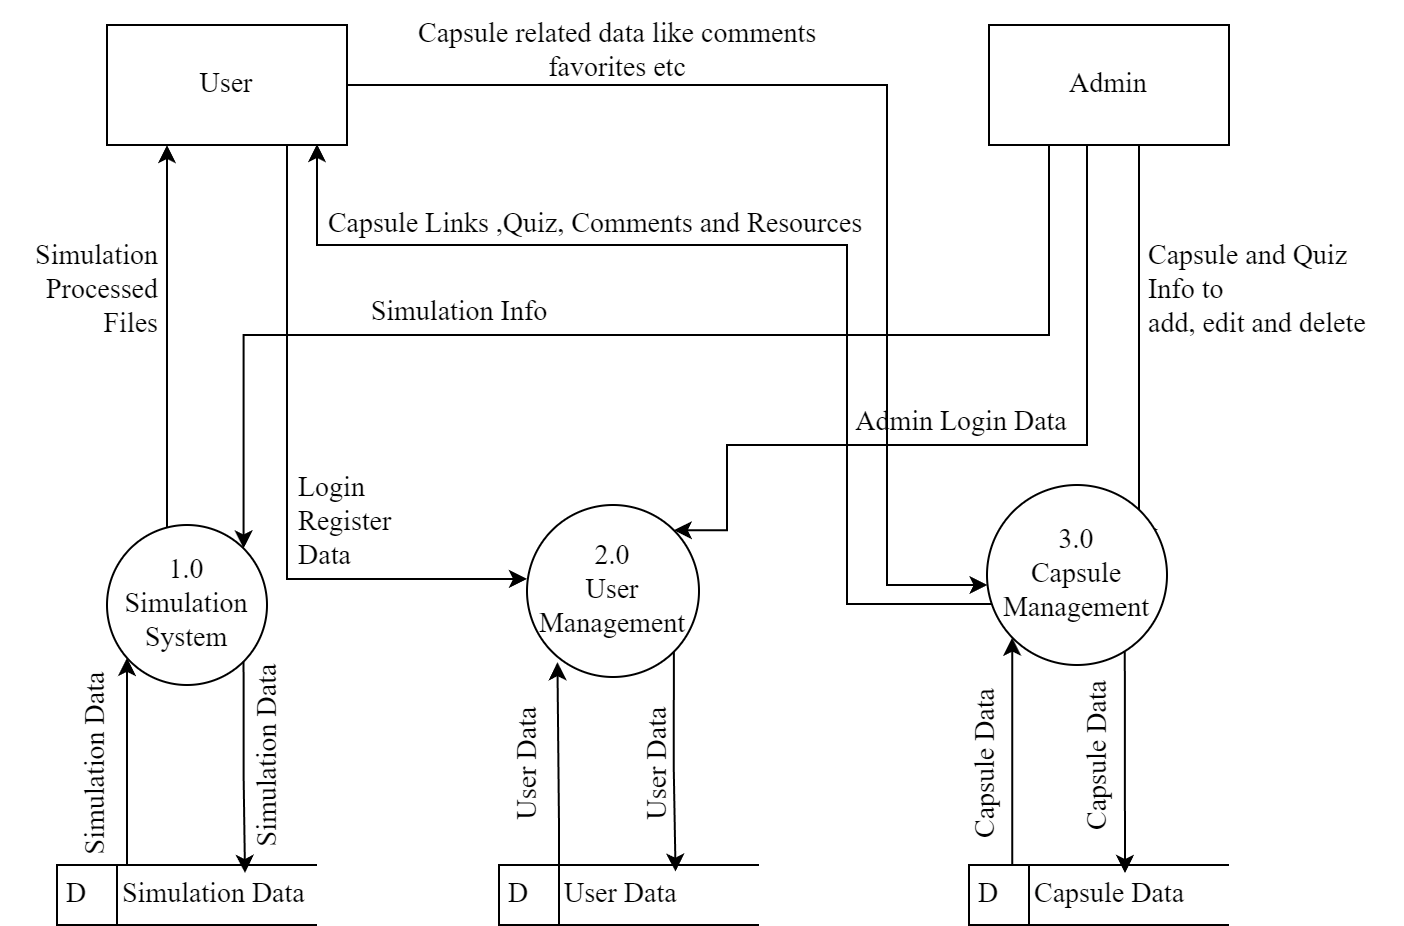
\includegraphics[width = 12.25cm]{Diagrams/Process 1.png}
    \caption{Process Model: DFD (Level 1)}
\end{figure}
\newpage
\textbf{Level 2 DFD}\\
These are even more detailed structure of flow of data into processes. In Level 2, Here it has more detailed view of each Processes above. Like 1.1 View Simulation is further divided from above 1 Simulation System Process.
\begin{figure}[H]
    \centering
        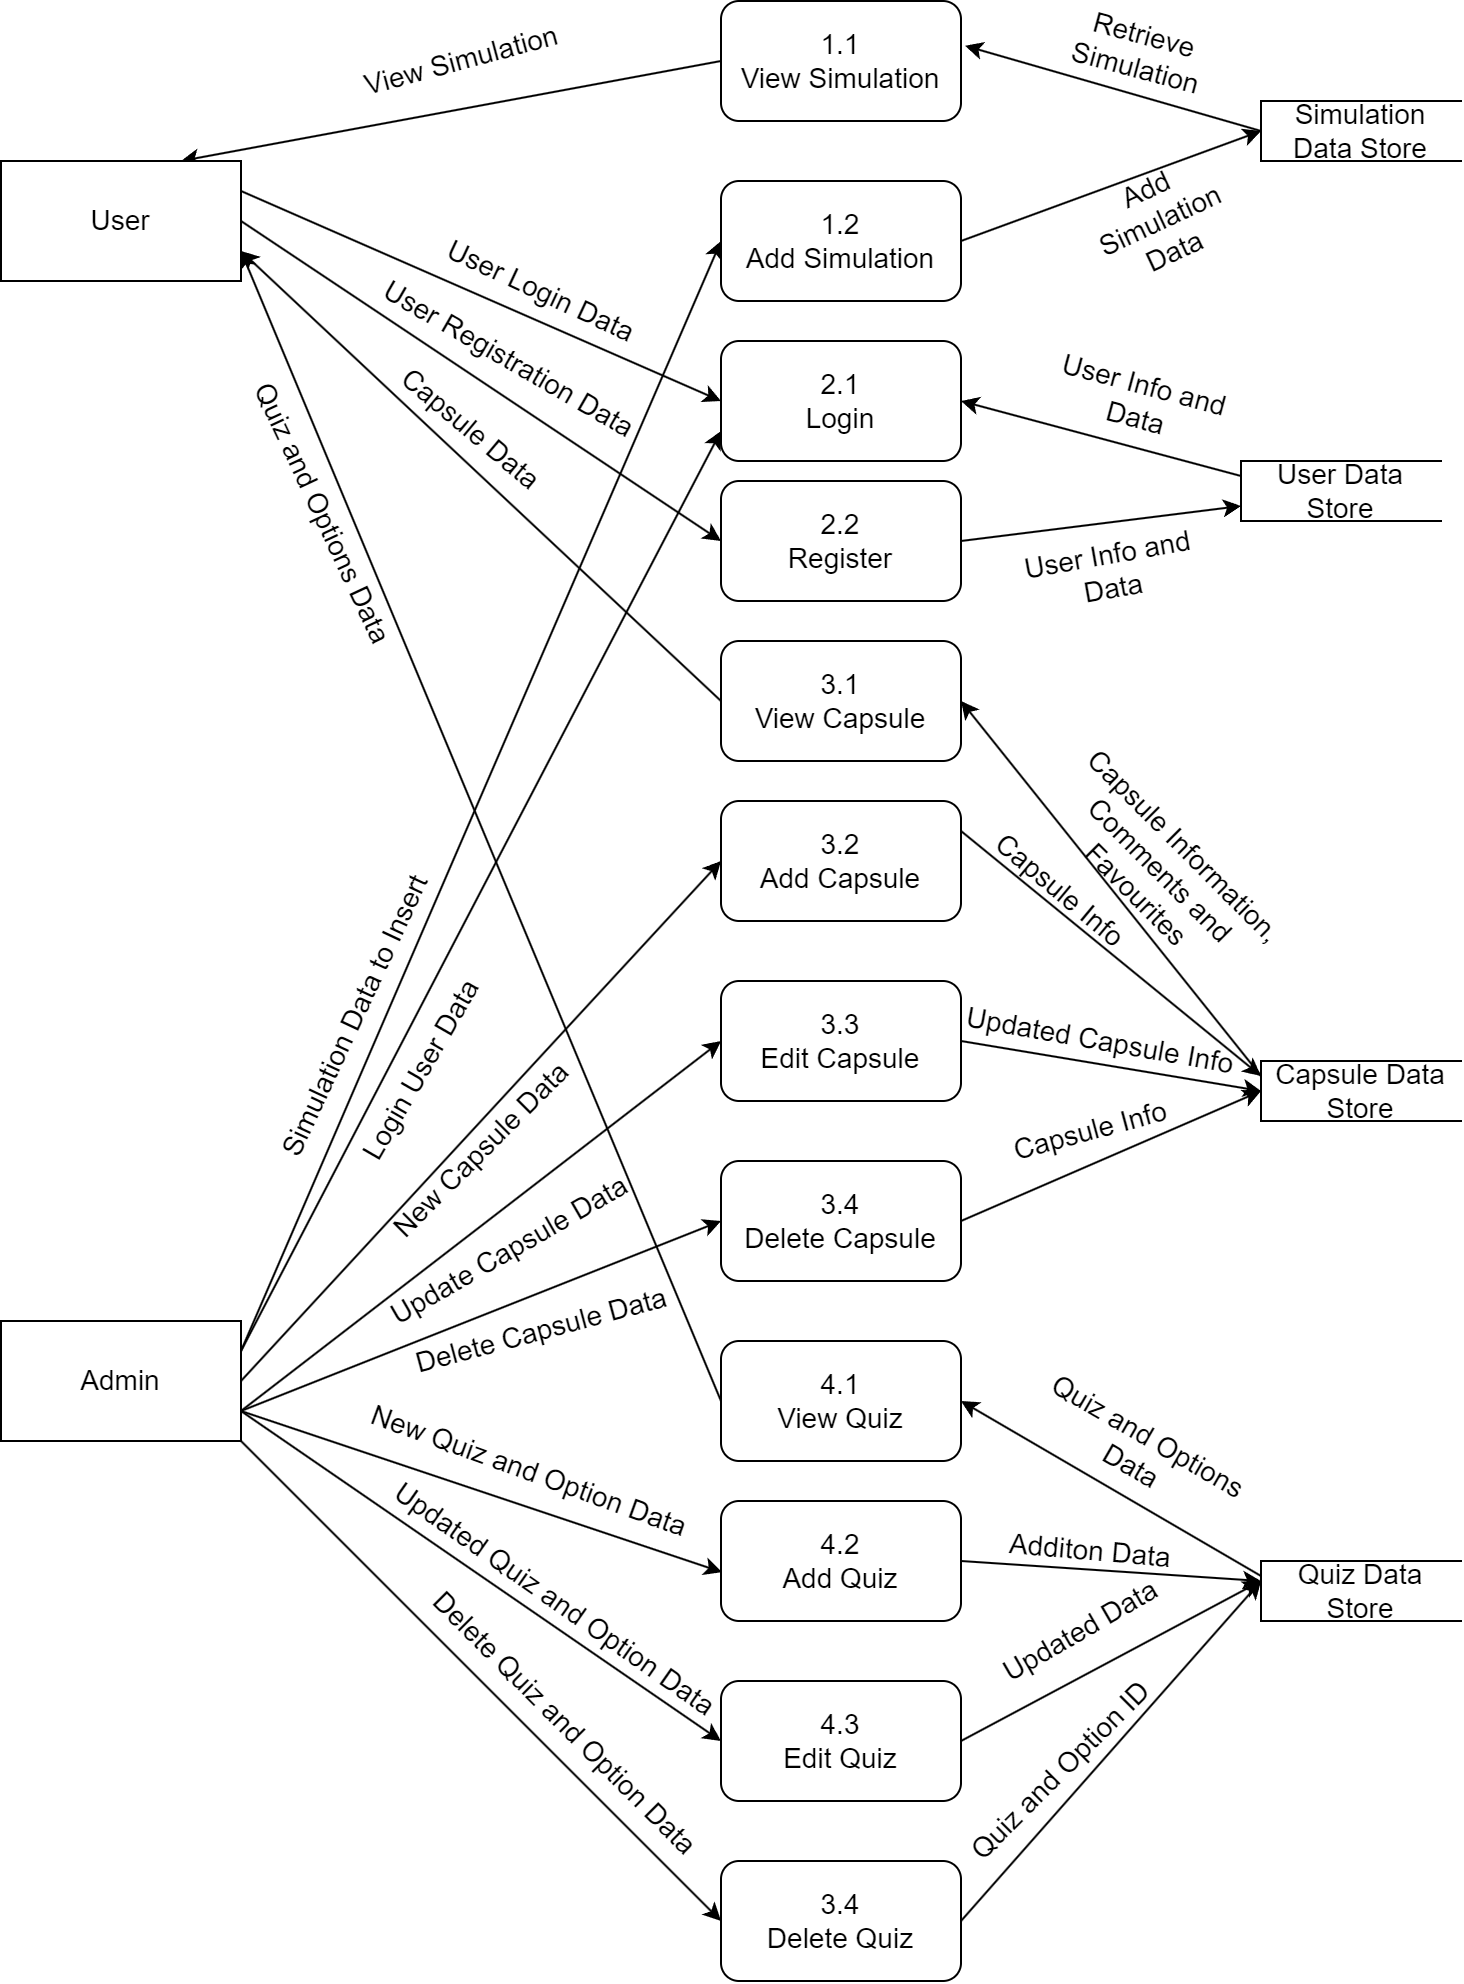
\includegraphics[width = 15cm]{Diagrams/Process3.png}
    \caption{Process Model: DFD (Level 2)}
\end{figure}
\newpage
\subsection{Data Modelling(ER-Diagram)}
The Entity-Relationship (ER) Diagram is primarily used to design a database schema. The ER diagram provided below facilitates the creation of a database in SQL by clearly illustrating the entities, their attributes, and the relationships between them. This visual representation helps in structuring the database effectively, ensuring that all necessary data elements and their interconnections are accounted for.
The system is organized into several key entities, each with specific attributes. 
\section*{Entities Description}
The Users entity represents the individuals who interact with the system, including attributes such as id, username, email, password, email\_verification\_token, and email\_verified to manage user authentication and verification. The Capsules entity covers various educational content units, each with a unique id, and attributes like title, description, thumbnail, images, pdf, category, and author\_id to provide detailed information and multimedia resources. Simulations are described by the Simulations entity, which includes id, title, description, link, and category to organize and access interactive simulations. The Comments entity enables user feedback on capsules, featuring attributes such as comment\_id, comment\_text, user\_id, and capsule\_id to link comments to their respective users and content. Quizzes, associated with capsules, are managed by the Quizzes entity, which includes quiz\_id, title, category, and capsule\_id for assessment purposes. The Options entity represents the various answers available for quizzes, with attributes such as option\_id, option\_text, is\_correct, and quiz\_id to identify and validate correct responses. Lastly, the Favorites entity tracks user preferences for capsules through user\_id and capsule\_id, enabling users to mark and easily access their favorite content.
\begin{figure}[H]
    \centering
    \rotatebox{90}{
        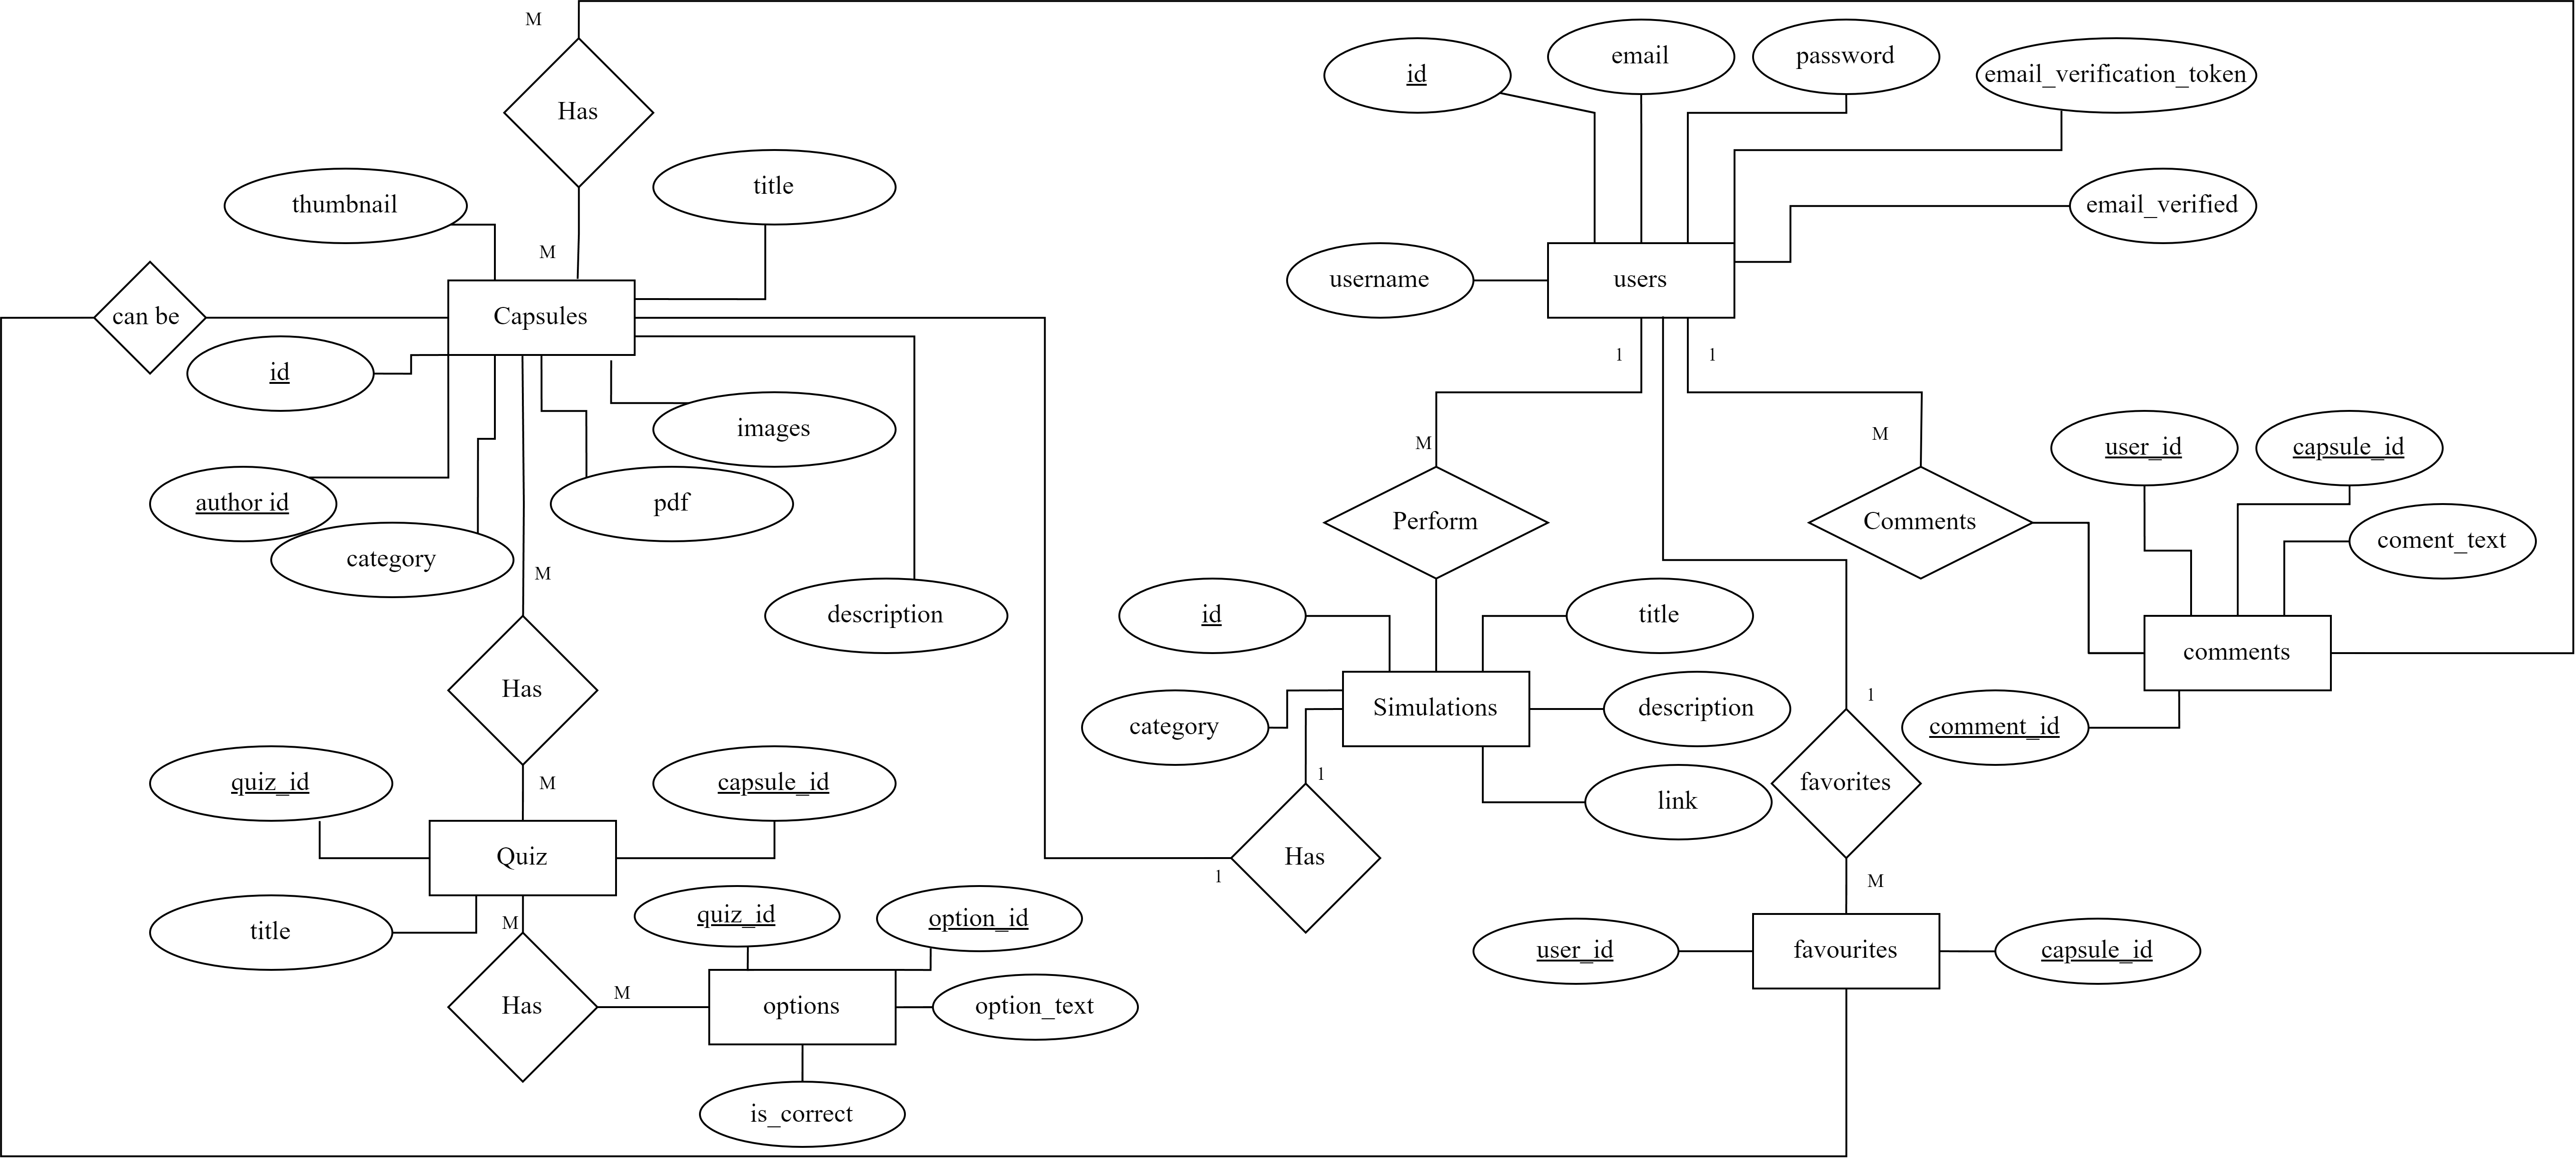
\includegraphics[height=10.8cm]{Diagrams/er.drawio.png}
    }
    \caption{ER Diagram of System Data}
\end{figure}
\newpage
\section{Structured System Design}
\subsection{Architecture Design}
The following diagram illustrates the architecture of our application. The application is structured using a three-tier architecture to ensure a clear separation of concerns and efficient functionality. The Presentation Layer, built with React.js, manages the user interface and user interactions. The Business Logic Layer, developed with Node.js and Express, handles core operations through middleware, routes, models, controllers, and utilities. Finally, the Data Management Layer uses PostgreSQL for relational database management and local server storage for handling files.
\begin{figure}[H]
    \centering
    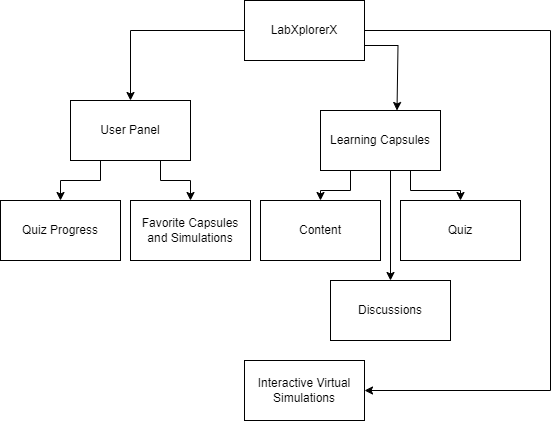
\includegraphics[height=16cm]{Diagrams/Main_Block.png}
    \caption{Three Tier Architecture of System}
\end{figure}
\newpage
\subsection{Database Schema Design}
The schema design details the tables, their attributes, and the relationships between them, ensuring that data is stored efficiently and consistently. This design includes defining primary keys to uniquely identify records, foreign keys to establish relationships between tables, and constraints to maintain data integrity. The schema design provides a clear blueprint for creating and managing the database, supporting effective data organization and retrieval as per the application’s requirements.
\begin{figure}[H]
   \centering
    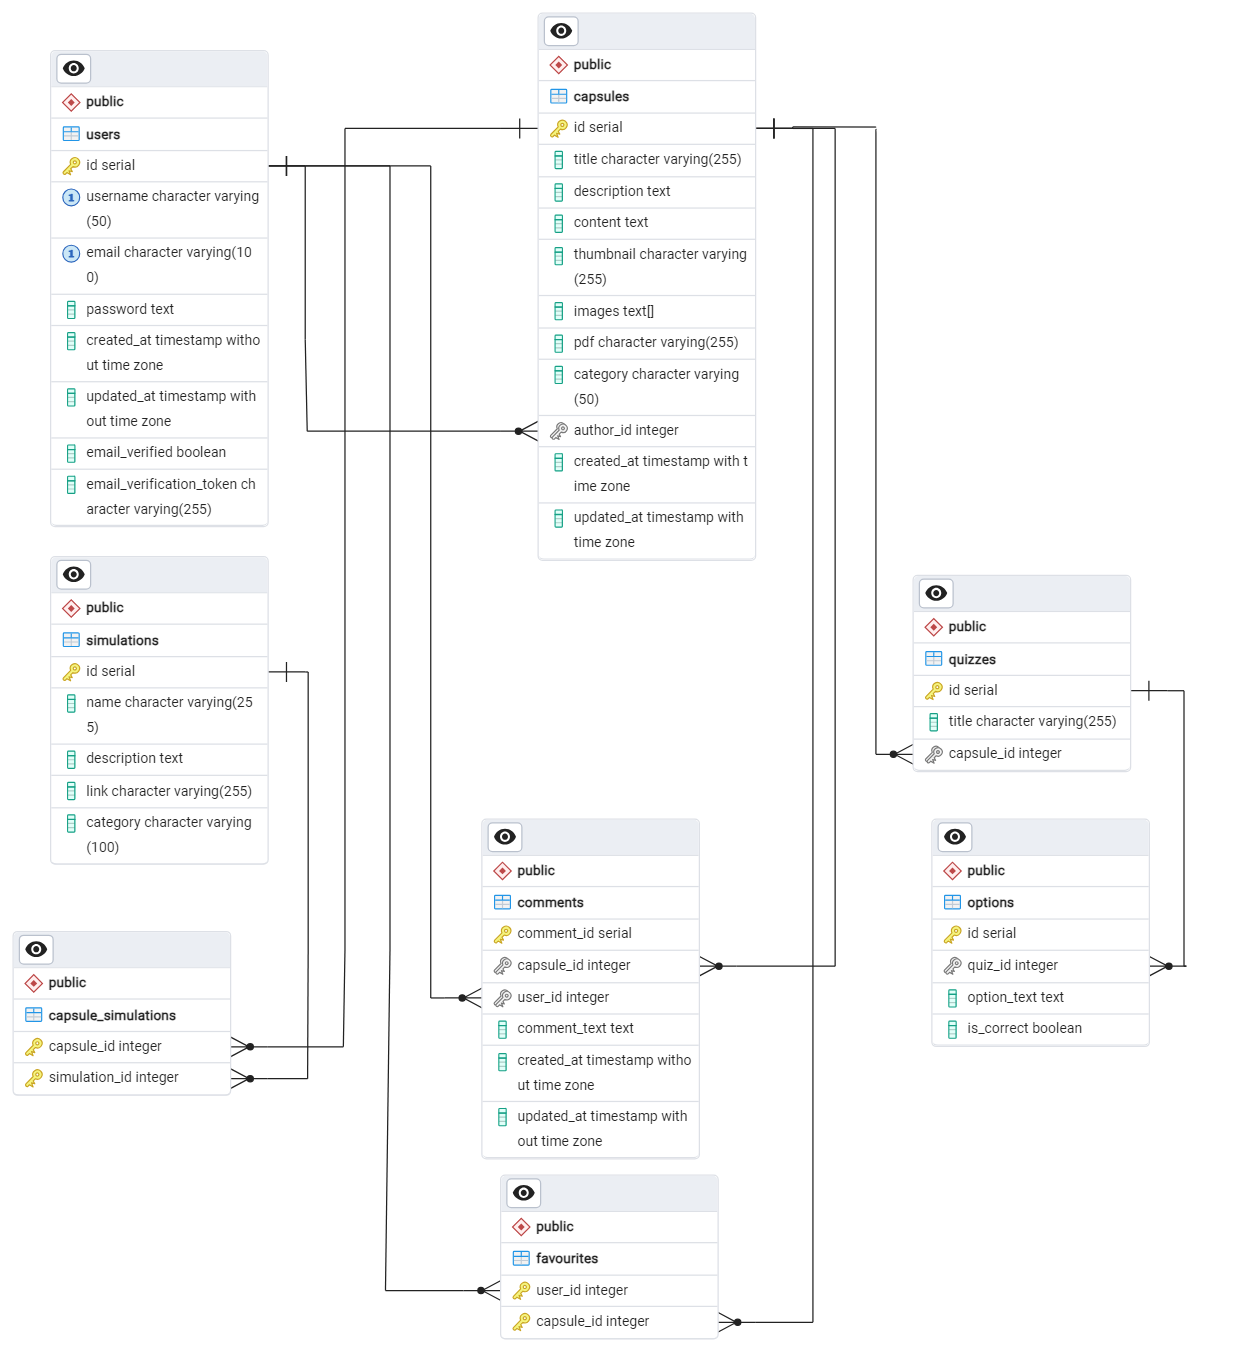
\includegraphics[height = 17cm]{Diagrams/Schema Design.png}
    \caption{Schema Design}
\end{figure}
\newpage
\subsection{Interface Design}
The interface design for this project focuses on creating a visually appealing, functional, and accessible user experience. The design includes layouts for essential screens such as the Home Screen, Menu, Capsule, Profile, and Admin Dashboard.

The main theme color chosen for the interface is Slate, a calm and professional color that provides consistency and a cohesive visual identity throughout the application. This choice ensures excellent readability and contrast with other UI elements, contributing to a clean and organized appearance.

For typography, the Poppins font is selected for its modern and clean look, which enhances readability across devices. Its uniform structure complements the minimalistic design, ensuring text remains legible and clear.

Button colors play an essential role in guiding user actions. A palette of Slate, Red, Green, and Blue is employed to differentiate between various actions. Slate is used for default or secondary actions, Red signals alerts or destructive actions, Green is for confirmation or positive actions like submissions, and Blue highlights primary actions such as saving or progressing to the next step.

Accessibility is a key consideration in the design. Buttons and interactive elements are designed to be large and clearly defined, making them easily distinguishable for users with visual impairments or motor difficulties. This promotes an inclusive experience, ensuring that all users can navigate and interact with the application comfortably.

Although the simulations are not responsive, the primary UI components have been optimized to ensure that essential elements scale properly on various devices, including desktops, tablets, and mobile screens. This responsiveness guarantees that the design maintains both usability and visual appeal across different screen sizes.

The design of buttons emphasizes usability, with large, easily clickable buttons that reduce the chance of misclicks and enhance overall user satisfaction. Their prominence ensures easy navigation, particularly on smaller devices or for users with accessibility needs.

Form design within the interface prioritizes clarity, validation, and accessibility. Each form field is accompanied by clear labels and placeholders, allowing users to understand the required input with ease. Real-time validation is implemented to provide immediate feedback, which helps users correct errors as they input data. Additionally, the form supports keyboard navigation, allowing users to move through fields efficiently using the tab key, a feature that enhances the accessibility of the form for users who rely on assistive devices.


\newpage
\subsection{Physical DFD}
A Physical Data Flow Diagram (DFD) provides a detailed view of how data flows through a system, focusing on physical components and their interactions. It illustrates the actual hardware, software, and network elements involved in processing and storing data. Unlike logical DFDs, which emphasize the functions and data flows abstractly, physical DFDs depict the real-world infrastructure, including servers, databases, and user interfaces.\\
Below is the Context Level DFD. 
\begin{figure}[H]
    \centering
    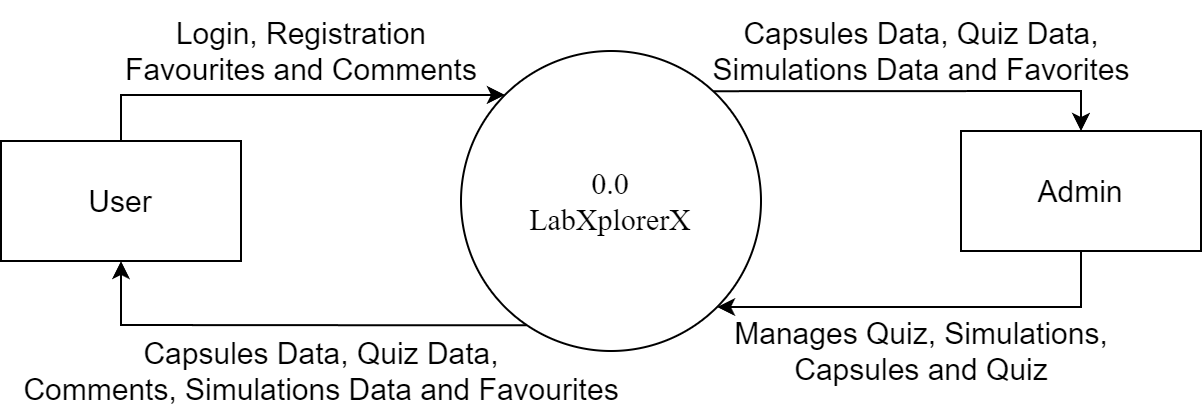
\includegraphics[height = 3cm]{Diagrams/physical0.png}
    \caption{Physical DFD (Context Level)}
\end{figure}
Below is the Level 1 DFD. Which shows detailed implementation of above Context Level DFD.
\begin{figure}[H]
    \centering
    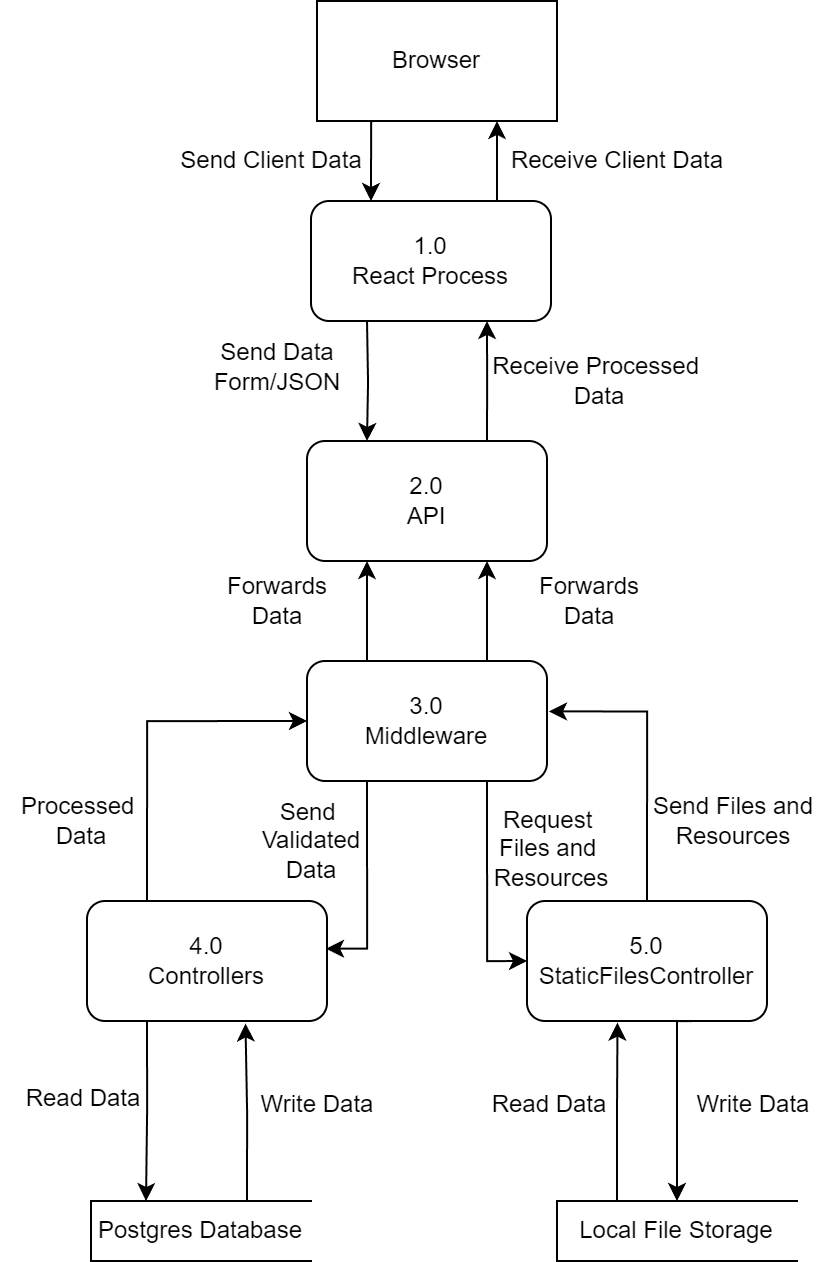
\includegraphics[height = 11cm]{Diagrams/physical1.png}
    \caption{Physical DFD (Level 1)}
\end{figure}
Below is the Level 2 DFD. Which shows us More Detailed implementation of Above processes and whats behind those processes. It shows how Frontend and Backend processes the data and data being flowed in the system.
\begin{figure}[H]
    \centering
    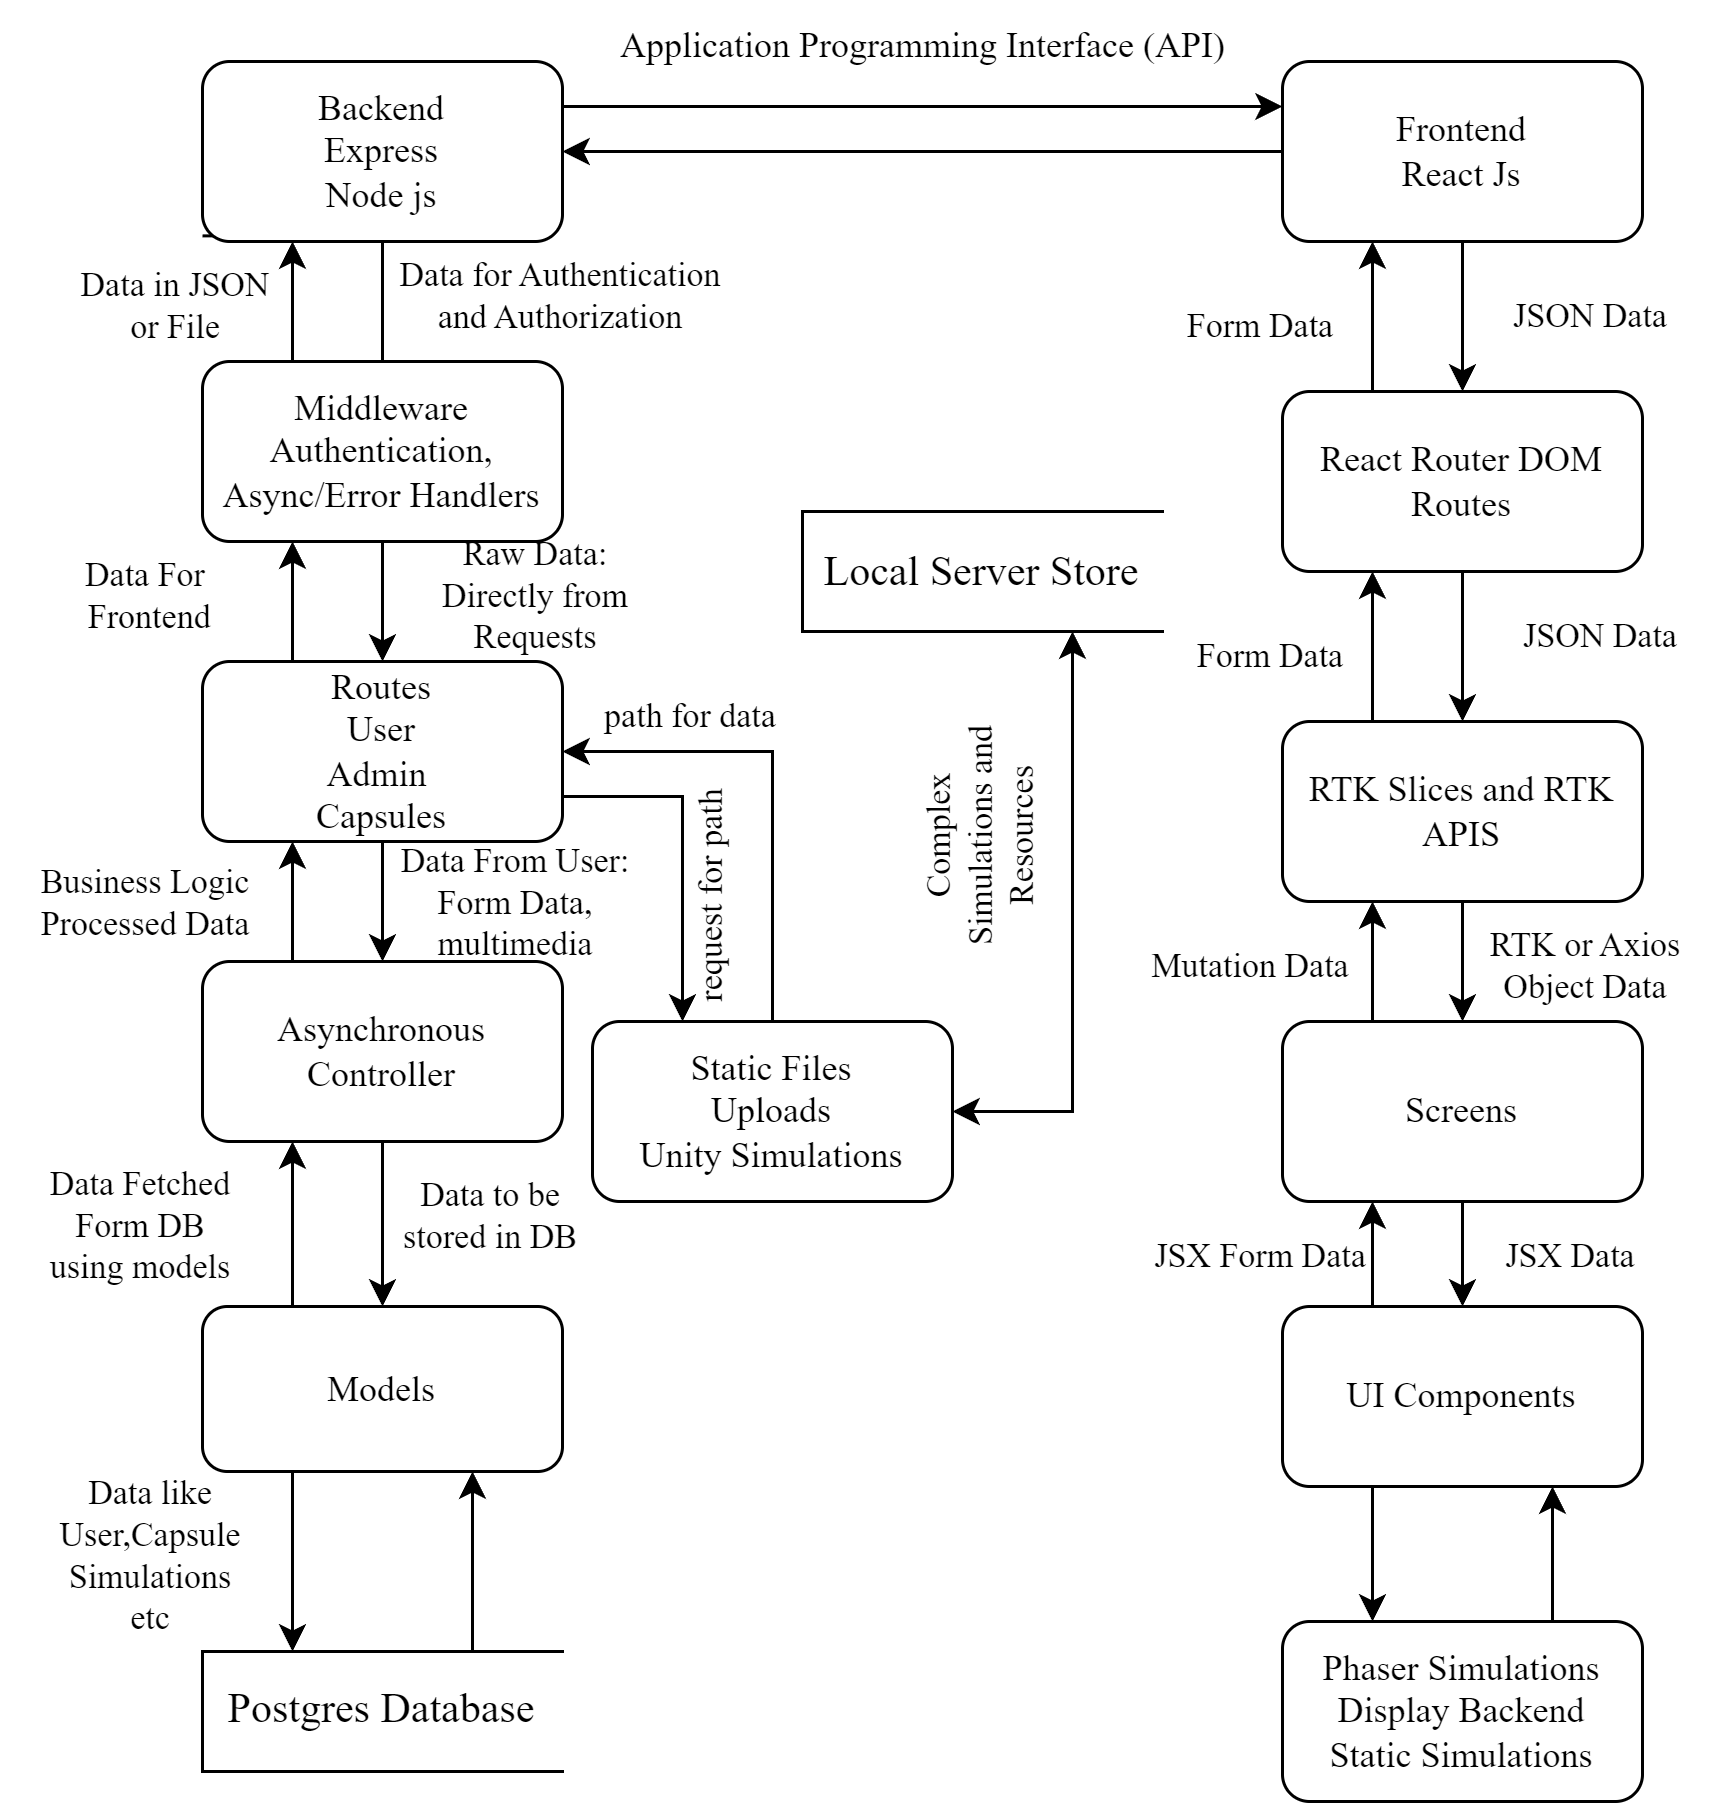
\includegraphics[height = 15cm]{Diagrams/DFD Process Modeling (1).png}
    \caption{Physical DFD (Level 2)}
\end{figure}
\newpage
\section{Algorithms}
\subsection{Simple Random Sampling Algorithm}
Simple Random Sampling algorithm is used in system to randomize quiz into the system. Through this algorithm we can select random set of quiz from large sample or set of data. Simple Random Sampling involves two main steps: shuffling the list and selecting the desired number of samples. Here are the details mentioned below:
\\
\textbf{Shuffling : Fisher-Yates shuffle}\\ To achieve randomness, the list is shuffled using an algorithm such as the Fisher-Yates shuffle. This algorithm has a time complexity of \( O(n) \), where \( n \) is the number of elements in the list. The Fisher-Yates shuffle works by iterating through the list once and swapping each element with another element chosen randomly from the remaining elements. This ensures each permutation of the list is equally likely.\\
 \textbf{Selection} \\After shuffling, the first \( k \) elements are selected where \( k \) is the number of desired samples. This step involves accessing \( k \) elements from the shuffled list, which has a time complexity of \( O(k) \).\\
\textbf{Overall Time Complexity} \\The total time complexity is the sum of the time complexities of shuffling and selection, which is \( O(n) \) for shuffling and \( O(k) \) for selection. Thus, the overall time complexity is \( O(n + k) \). In practical scenarios, if \( k \) is much smaller than \( n \), this can be simplified to \( O(n) \) as the term \( O(k) \) becomes negligible in comparison to \( O(n) \).\\
\textbf{Algorithm:}
\vspace{-\baselineskip}
\begin{enumerate}
    \item \textbf{Shuffling:}For each element in the list, from the first to the second-to-last (i.e., from index 0 to \( n-2 \)):
        \begin{itemize}
            \item Generate a random index \( j \) such that \( j \) is between the current index \( i \) and the last index \( n-1 \).
            \item Swap the element at index \( i \) with the element at index \( j \).
        \end{itemize}
    \item \textbf{Selection:} After shuffling, select the first \( k \) elements from the shuffled list.
    \item \textbf{Output:} The selected \( k \) elements as the random sample.
\end{enumerate}

% \section{Algorithm Details}